% $Header$

\documentclass{beamer}

% Copyright (c)  2021  HiKlas Ltd.
% Permission is granted to copy, distribute and/or modify this document
% under the terms of the GNU Free Documentation License, Version 1.3
% or any later version published by the Free Software Foundation;
% with no Invariant Sections, no Front-Cover Texts, and no Back-Cover Texts.
% A copy of the license is included in the section entitled "GNU
% Free Documentation License".
%
% Based on the Beamer generic-ornate-15min-45min.en.tex template by
% Till Tantau <tantau@users.sourceforge.net>



\mode<presentation>
{
  \usetheme{CambridgeUS}
}

\usepackage[english]{babel}
\usepackage[latin1]{inputenc}
\usepackage[T1]{fontenc}
% Or whatever. Note that the encoding and the font should match. If T1
% does not look nice, try deleting the line with the fontenc.

% These packages are used for drawing circuits
\usepackage{tikz}
\usepackage[siunitx,european,americanresistors]{circuitikz}

% Packages for mathematical notation
\usepackage{amsmath}

% Trying to split long URLs across lines
% From this post suggesting breakurl: https://stackoverflow.com/questions/2640111/url-latex-linebreak
% The breakurl package: https://ctan.org/pkg/breakurl?lang=en
% Example of options: https://tex.stackexchange.com/questions/298851/linebreak-in-long-url-breakurl-wont-break-it
\usepackage{hyperref}
\usepackage[hyphenbreaks]{breakurl}


% Information about the presentation 
\title{Introduction to Machine Code}
\subtitle{003 6502 CPU}
\author{Fiona Bianchi}
\institute{HiKlas Ltd}
\date{August 2021}
\subject{Talks}
\pgfdeclareimage[height=0.5cm]{company-logo}{../assets/HiklasLogo.eps}
\logo{\pgfuseimage{company-logo}}

% Table of contents for each Subsection
\AtBeginSubsection[]
{
  \begin{frame}<beamer>{Outline}
    \tableofcontents[currentsection,currentsubsection]
  \end{frame}
}

% TODO: Nope, I don't think I want this put leaving it in just in case
% TODO: to remove when absolutely sure
% If you wish to uncover everything in a step-wise fashion, uncomment
% the following command: 
%\beamerdefaultoverlayspecification{<+->}

% Show the notes
\ifdefined\isnotes
  \setbeameroption{show only notes}
\fi

% Show notes and slides
\ifdefined\ishandout
\setbeameroption{show notes}
\fi

\begin{document}

\begin{frame}
  \titlepage
\end{frame}

\begin{frame}{Outline}
  \tableofcontents
  % TODO: What is "pausesections" for?
  % You might wish to add the option [pausesections]
\end{frame}


\section{6502 Central Processor Unit}

\subsection[History]{History}

\begin{frame}{A frame}
  \begin{itemize}
  \item
    One item
  \item
    Two item
  \end{itemize}
\end{frame}


\subsection[Appearance]{What does it look like?}

\begin{frame}{Chip Pinout}
  \begin{columns}
    \column{0.50\textwidth}
    \begin{itemize}
    \item
      Pinout diagrams show the connections into the chip die
    \item
      There are signals for data, address, control lines as well as power
    \item
      Importanly the chip also has several clock connections
    \end{itemize}

    \column{0.50\textwidth}
    \begin{center}
      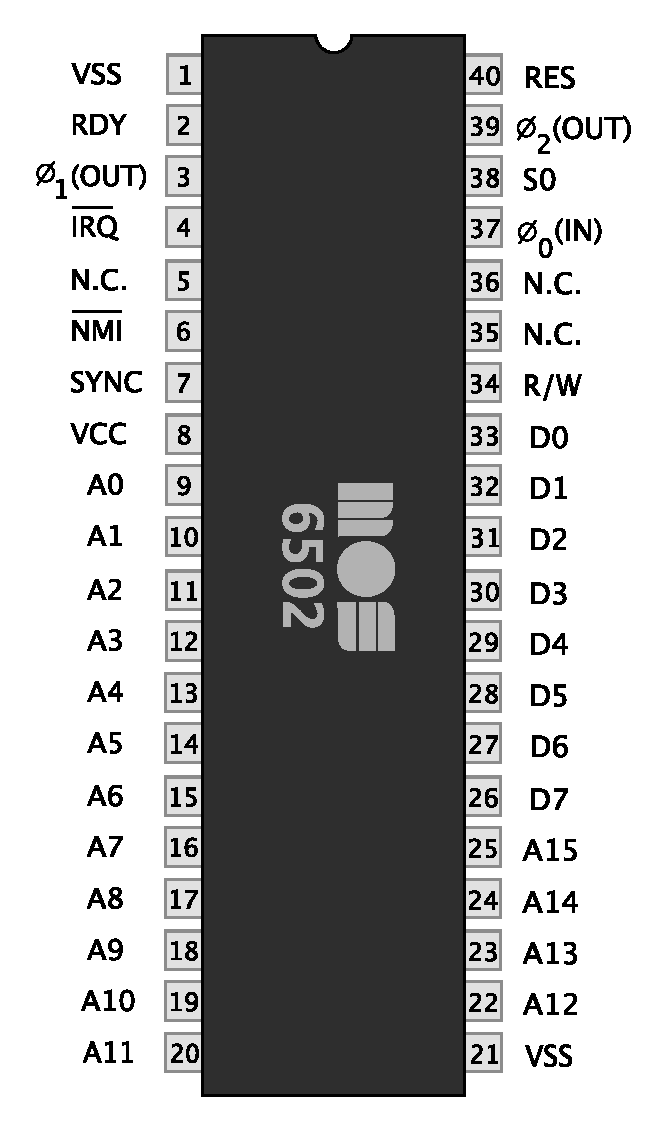
\includegraphics[scale=0.25]{../assets/MOS6502.eps}
      \cite{MOS6502Chip} Chip Pinout Diagram
    \end{center}
    
  \end{columns}
\end{frame}

\begin{frame}{Chip Die}
  \begin{columns}
    \column{0.5\textwidth}
    \begin{itemize}
    \item
      One item
    \item
      Two item
    \end{itemize}

    \column{0.5\textwidth}
    \begin{center}
      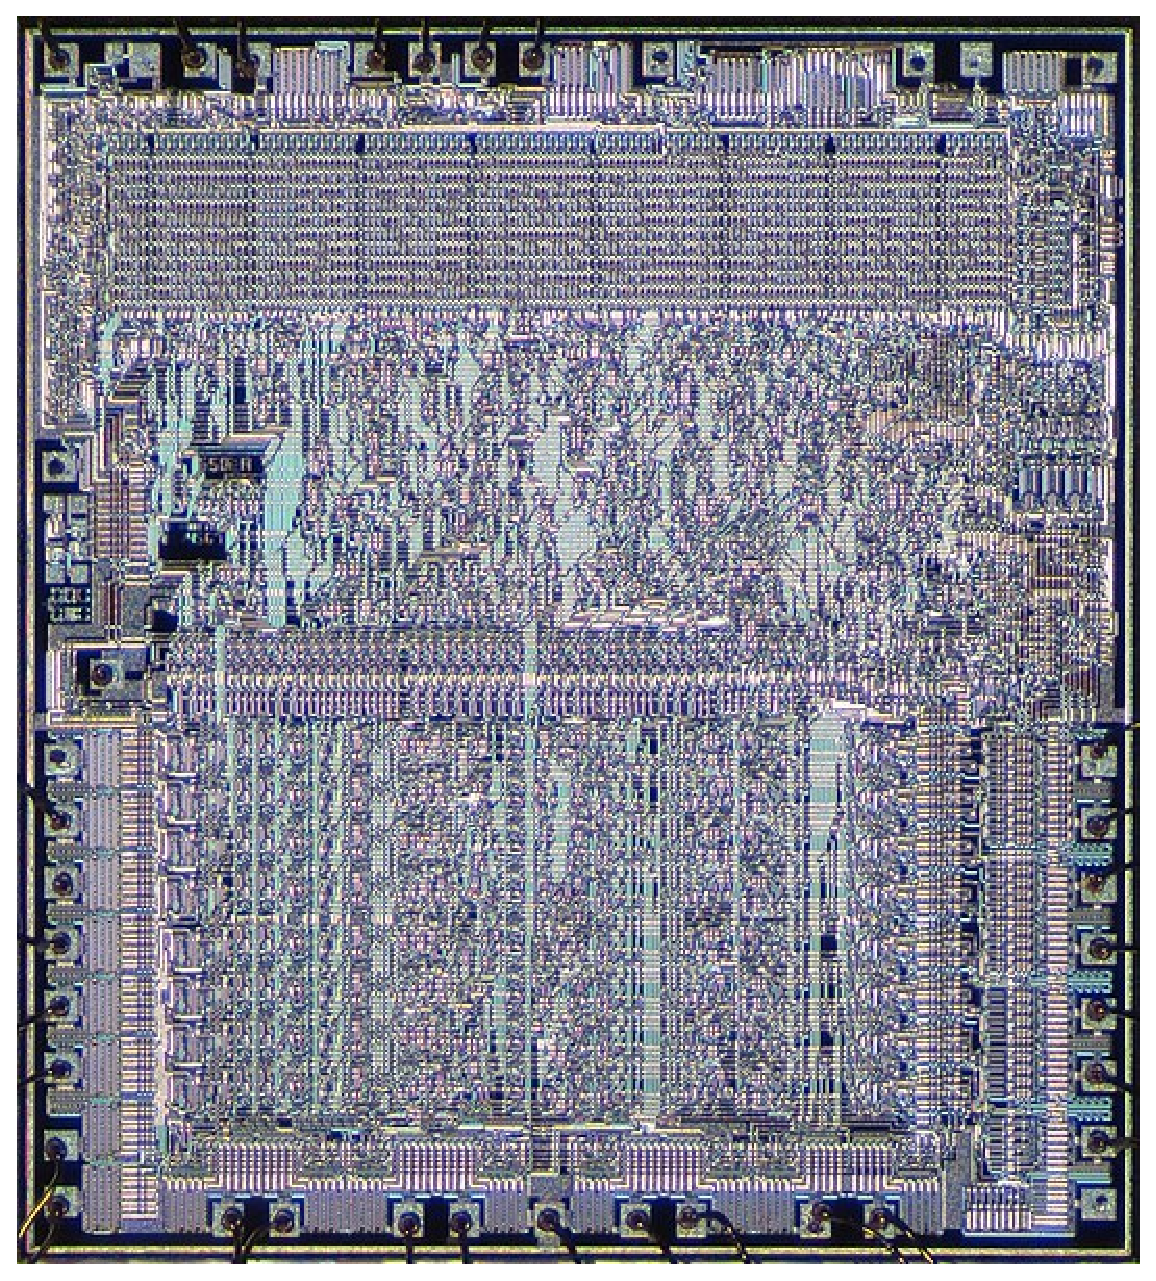
\includegraphics[scale=0.25]{../assets/MOS_6502_die.eps}
      \cite{MOS6502Die} The piece of silicon wafer 

    \end{center}
  \end{columns}
\end{frame}


\subsection[Internals]{What's inside?}

\begin{frame}{Architecture}
  \begin{itemize}
  \item
    Registers
    \begin{itemize}
    \item
      A - Accumulator
    \item
      X
    \item
      Y - Index Register
    \end{itemize}
  \item
    P - Status Register
  \item
    PC - Program Counter
  \item
    SP - Stack Pointer
  \end{itemize}
\end{frame}

\begin{frame}{Accumulator}
  \begin{itemize}
  \item
    Destination for mathematical operations
  \item
    Source for logic and other operations
  \item
    Operations on accumulator impact status register
  \end{itemize}
\end{frame}


\section{Programming}

\subsection[Instructions]{Instructions}

\begin{frame}{A frame}
  \begin{itemize}
  \item
    One item
  \item
    Two item
  \end{itemize}
\end{frame}


\subsection[Interupts]{Getting interrupted}

\begin{frame}{A frame}
  \begin{itemize}
  \item
    One item
  \item
    Two item
  \end{itemize}
\end{frame}


\section{Emulator}

\subsection[GettingStarted]{Getting Started}

\begin{frame}{A frame}
  \begin{itemize}
  \item
    One item
  \item
    Two item
  \end{itemize}
\end{frame}

\subsection[Examples]{Example Code}

\begin{frame}{A frame}
  \begin{itemize}
  \item
    One item
  \item
    Two item
  \end{itemize}
\end{frame}




\section{Summary}

\begin{frame}{Summary}

  % Keep the summary *very short*.
  \begin{itemize}
  \item
    Item one
  \item
    Item two
  \end{itemize}
  
  % The following outlook is optional.
  \vskip0pt plus.5fill
  \begin{itemize}
  \item
    Outlook
    \begin{itemize}
    \item
      Something you haven't solved.
    \item
      Something else you haven't solved.
    \end{itemize}
  \end{itemize}
\end{frame}

\section{Bibliogrphy}

\begin{frame}{Bibliography 1}
  \frametitle{References}

  % The label is just to indicate the longest test that
  % needs to be laid out in the bibliography 
  \begin{thebibliography}{6502 Wikipedia Page}
  \bibitem[MOS 6502 Die]{MOS6502Die}
    Die image
    \newblock {\url{https://commons.wikimedia.org/wiki/File:MOS_6502_die.jpg}}
    
  \bibitem[MOS 6502 Chip]{MOS6502Chip}
    Chip image
    \newblock {\url{https://commons.wikimedia.org/wiki/File:MOS6502.svg}}

  \bibitem[6502 Wikipedia Page]{6502Wikipedia}
    6502 Wikipedia Page
    \newblock {\url{https://en.wikipedia.org/wiki/MOS_Technology_6502}}

  \end{thebibliography}
\end{frame}


\end{document}


